\documentclass[tikz,border=10pt]{standalone}

\usepackage{xcolor}
\usetikzlibrary{
    arrows.meta,
    positioning,
    fit,
    backgrounds
}

\begin{document}

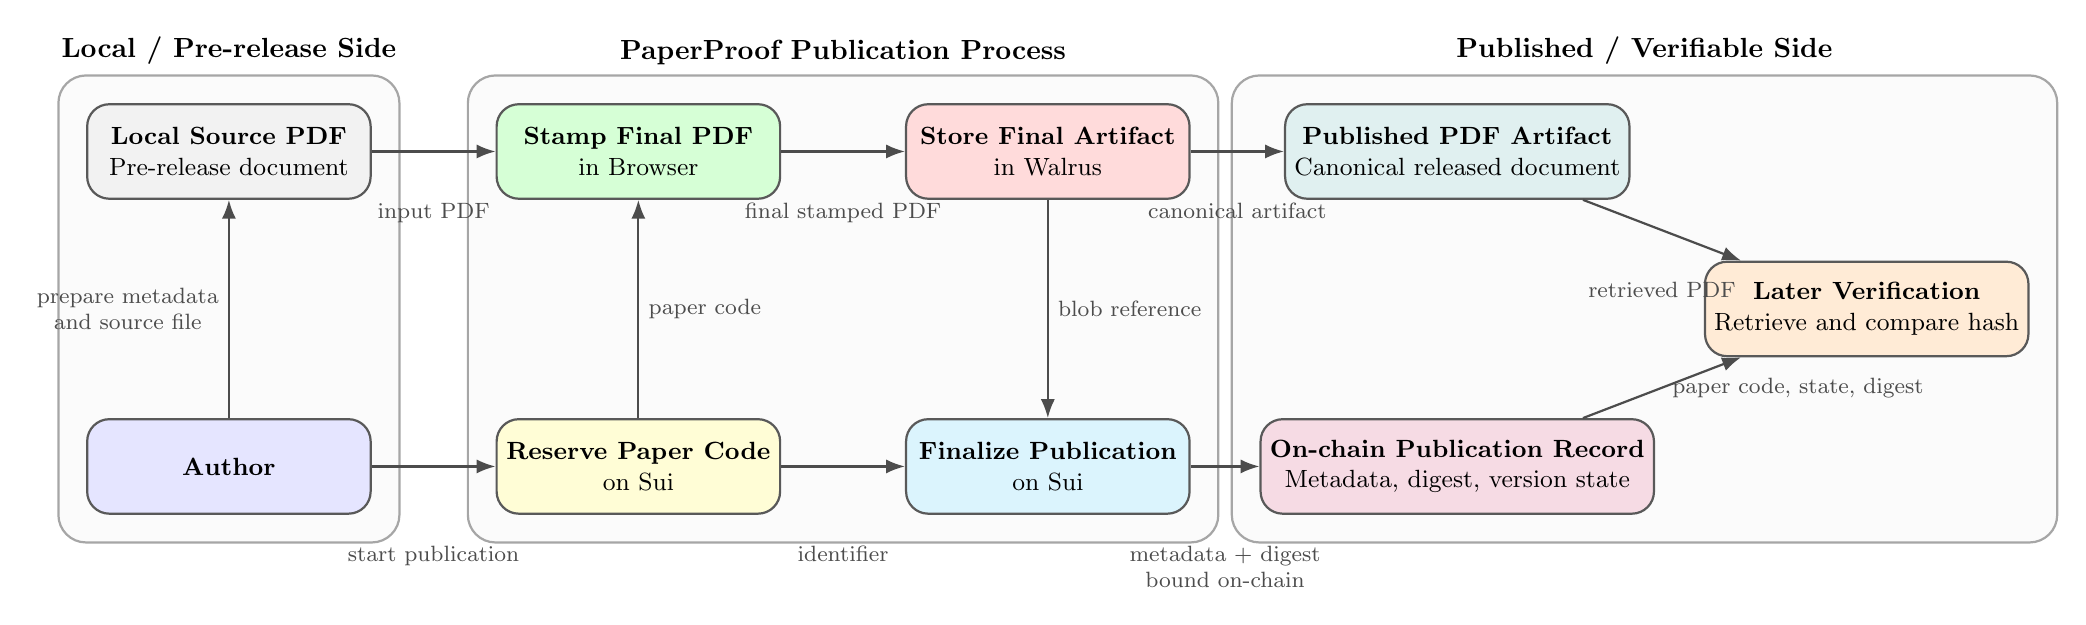
\begin{tikzpicture}[
    font=\small,
    box/.style={
        rectangle,
        rounded corners=8pt,
        draw=black!65,
        thick,
        align=center,
        minimum width=3.6cm,
        minimum height=1.2cm,
        fill=white
    },
    arrow/.style={
        -{Latex[length=2.4mm,width=1.8mm]},
        thick,
        draw=black!70
    },
    note/.style={
        font=\footnotesize,
        align=center,
        text=black!70
    },
    layer/.style={
        rectangle,
        rounded corners=10pt,
        draw=black!35,
        thick,
        fill=gray!3,
        inner sep=10pt
    }
]

% =========================================================
% Left: local / pre-release side
% =========================================================
\node[box, fill=blue!10] (author) at (0,0)
{\textbf{Author}};

\node[box, fill=gray!10] (localpdf) at (0,4)
{\textbf{Local Source PDF}\\Pre-release document};

% =========================================================
% Middle: PaperProof publication model
% =========================================================
\node[box, fill=yellow!16] (reserve) at (5.2,0)
{\textbf{Reserve Paper Code}\\on Sui};

\node[box, fill=green!16] (stamp) at (5.2,4)
{\textbf{Stamp Final PDF}\\in Browser};

\node[box, fill=red!14] (walrus) at (10.4,4)
{\textbf{Store Final Artifact}\\in Walrus};

\node[box, fill=cyan!14] (finalize) at (10.4,0)
{\textbf{Finalize Publication}\\on Sui};

% =========================================================
% Right: published / verifiable side
% =========================================================
\node[box, fill=teal!12] (publishedpdf) at (15.6,4)
{\textbf{Published PDF Artifact}\\Canonical released document};

\node[box, fill=purple!14] (record) at (15.6,0)
{\textbf{On-chain Publication Record}\\Metadata, digest, version state};

\node[box, fill=orange!16] (verify) at (20.8,2)
{\textbf{Later Verification}\\Retrieve and compare hash};

% =========================================================
% Background groups
% =========================================================
\begin{scope}[on background layer]
\node[layer,
    fit=(author)(localpdf),
    label={[font=\bfseries]north:Local / Pre-release Side}
] {};

\node[layer,
    fit=(reserve)(stamp)(walrus)(finalize),
    label={[font=\bfseries]north:PaperProof Publication Process}
] {};

\node[layer,
    fit=(publishedpdf)(record)(verify),
    label={[font=\bfseries]north:Published / Verifiable Side}
] {};
\end{scope}

% =========================================================
% Arrows
% =========================================================
\draw[arrow] (author) -- node[left, note] {prepare metadata\\and source file} (localpdf);

\draw[arrow] (author.east) -- node[below, yshift=-25pt, note] {start publication} (reserve.west);
\draw[arrow] (localpdf.east) -- node[below, yshift=-15pt, note] {input PDF} (stamp.west);

\draw[arrow] (reserve) -- node[right, note] {paper code} (stamp);
\draw[arrow] (stamp) -- node[below, yshift=-15pt, note] {final stamped PDF} (walrus);
\draw[arrow] (reserve) -- node[below, yshift=-25pt, note] {identifier} (finalize);
\draw[arrow] (walrus) -- node[right, note] {blob reference} (finalize);

\draw[arrow] (finalize) -- node[below, yshift=-25pt, note] {metadata + digest\\bound on-chain} (record);
\draw[arrow] (walrus) -- node[below, yshift=-15pt, note] {canonical artifact} (publishedpdf);

\draw[arrow] (record) -- node[right, note] {paper code, state, digest} (verify);
\draw[arrow] (publishedpdf) -- node[below, yshift=-15pt, note] {retrieved PDF} (verify);

\end{tikzpicture}

\end{document}
